 The proposed biomechanical model consist of two bodies, one representing the pectoral cage  and the second represents the breast soft tissues. Between the two bodies, a contact surface is defined in order to model tissues mechanics at the juncture interface.
 
The next section describes the implementation of different interaction models tested during the model development process. Since the breast tissues are always attached to the pectoral muscle (Figure \ref{fig:contactsurface}), the contact surface was modeled using \textit{bonded} and \textit{no-separation frictional} interaction models only.

\begin{figure}[!h]
\centering
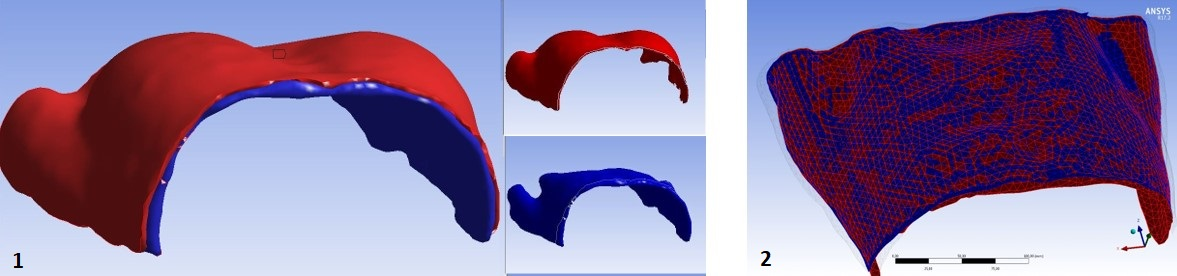
\includegraphics[width=0.9\textwidth,keepaspectratio]{figures/contactSurface.jpg} 
\caption{The two bodies representing the thoracic cage and breast with the associated contact surface.  Blue surface- the target surface, red surface - contact surface}
\label{fig:contactsurface}
\end{figure}

The results for pure bonded and pure no-separation sliding models as well as one combined contact surface are listed bellow. For some contacts models, because of important solution instabilities or a poor fidelity to the real breast mechanics,only partial results are presented.  

\subsubsection*{Bonded contact surface}

First a pure bounded contact was used to model the interaction between the breast and the muscle. To achieve realistic breast deformation extremely low values of equivalent Young's modulus and Poisson ratio were needed ($\lambda_{breast} = 0.3kPa$ and $\nu_{breast} = 0.45$).  
An example of breast deformation in prone and supine configuration is illustrated in Figure \ref{fig:bondedcontact}.

\begin{figure}[!h]
\centering
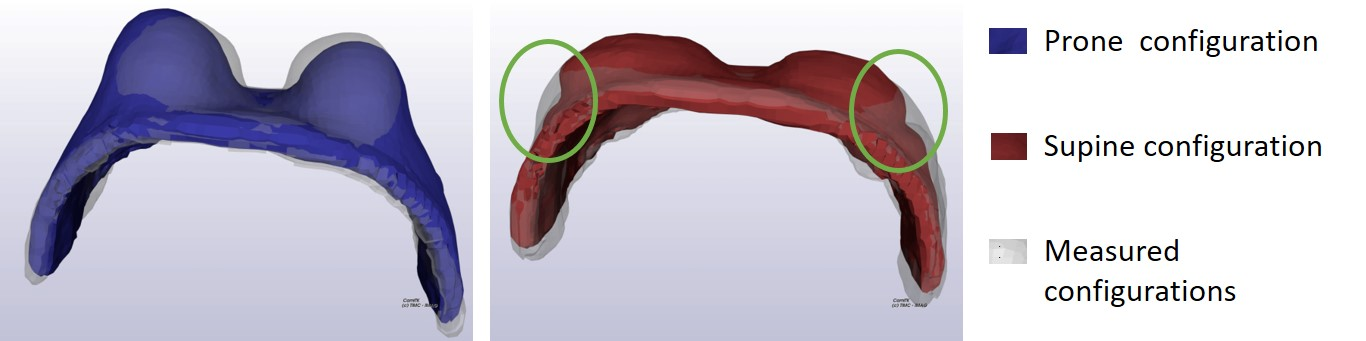
\includegraphics[width=0.9\textwidth,keepaspectratio]{figures/bondedcontact.jpg} 
\caption{Resulting breast deformation with a bonded contact model.}
\label{fig:bondedcontact}
\end{figure}

One can see that, even if the breast geometry in prone position is well estimated, the one in supine and supine tilted configurations are constrained laterally. Moreover, a important volume variation was observed which is not a characteristic of breast changes under gravity loading. The volume variation is due to a low value of the Poisson ratio. 

\subsubsection*{Sliding contact surface}

Pure sliding contact surface was considered in order to allow more tissues displacement on lateral direction. The breast sliding over the muscle surface was modeled using the Coulomb friction low (Section \ref{subsection:surfaceinteractionmodels}). Additional boundary condition were set by imposing zero-displacement on the right, left, superior and inferior mesh boundaries representing the breast volume (see Figure \ref{fig:meshboundaries} for a recall on different mesh boundaries).  This model caused large convergence problems because of breast tissues over-sliding. It was obvious that the model needs more boundary conditions in order to archive convergence. Moreover a non-linear and a non-uniform sliding model was needed in order imitate the behavior of rich fibrous areas where the breast is attached to the chest wall ( see Section \ref{subsection:internalstructures} for a recall on breast anatomy). 


\subsubsection*{Mixt contact surface}

In order to limit breast tissues sliding a mixt contact surface is defined. Herein, the contact surface consist of two complementary areas (Figure \ref{fig:mixtcontact}), one modeled as bounded contact and the second one modeled as no-separation sliding contact. The regions corresponding to the bounded contact are defined following the anatomical structures were the concentration of fibrous tissues is significantly high. Such regions are encountered along the muscle surface where the superficial muscle fascia meets the breast suspensory ligaments as the inframammary ligament, deep medial ligament or deep lateral ligament.

\begin{figure}[!h]
\centering
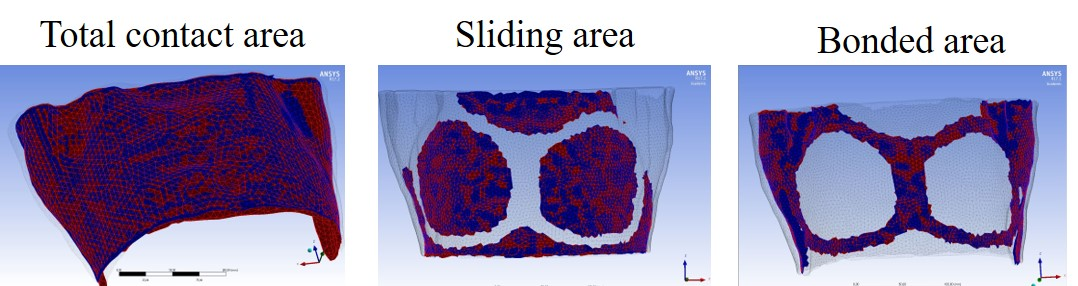
\includegraphics[width=0.9\textwidth,keepaspectratio]{figures/mixtcontactarea.jpg} 
\caption{The contact surface divided in two regions: sliding region and bonded region.}
\label{fig:mixtcontact}
\end{figure}

Using such a contact model have improved substantially the estimate of the supine breast configuration. However because of a high deformation gradient imposed at the juncture border between the two contact areas, solution convergence problems were meet. Moreover, then the supine configuration is estimated, several fold are created at the skin surface (Figure \ref{fig:mistcontactresults}). Same type of fold were obtained in supine tilted configuration creating large convergence problems because of tissues superposition.

\begin{figure}[!h]
\centering
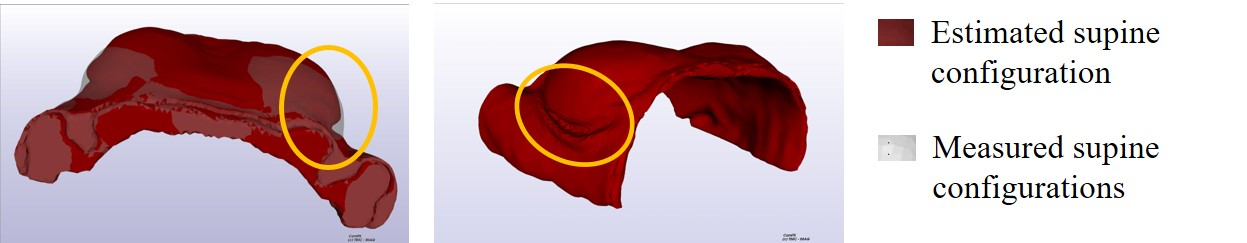
\includegraphics[width=0.9\textwidth,keepaspectratio]{figures/mixt_contact_supine.jpg} 
\caption{The contact surface divided in two regions: sliding region and bonded region.}
\label{fig:mistcontactresults}
\end{figure}

The last described model have provided satisfactory results, however its implies important solution convergence problems. Therefore, the model was improved by replacing the bonded contact regions with stiff ligaments connecting the breast tissues to the muscle.  Contrary to the bonded contact, the ligaments preclude progressively the breast tissues from sliding and allows a slight displacement avoiding the folds creation. Moreover, an additional layer modeling the deep layer of breast superficial fascia was added at the juncture surface between breast and muscle. Knowing that the fascia is stiffer than the breast soft tissues its control the amount of sliding and facilitate the solution convergence. For more information on ligaments and fascia mechanical properties see the Section \ref{section:myBoundayconditions}.